% Required packages in the main preamble:
% \usepackage{graphicx}
% \usepackage{booktabs}
% \usepackage{array}

\providecommand{\SysName}{CARE}

\section{Evaluation}
\label{sec:evaluation}

We evaluate \SysName{} on a large-scale C/C++ benchmark and report the strongest
completed experimental setting: full-project opportunity detection over OSS50
and real LLM patch generation plus validation for all critical
resource-lifecycle findings. We use this setting because it exercises the full
pipeline end to end, targets security-relevant refactoring opportunities, and
has complete results for both \SysName{} and a direct LLM-only baseline. The
evaluation focuses on accepted patches: a candidate contributes to the final
yield only if it applies to the real project, survives build/test and static
checks where available, and passes the resource, semantic, and security
regression gates. We ask four questions:

\noindent\textbf{RQ1.} Can \SysName{} generate patches that apply and pass
validation more often than direct LLM-only patching?
\textbf{RQ2.} Which validation components are necessary to avoid unsafe
acceptance?
\textbf{RQ3.} Among patches accepted by the validator, how often do they appear
correct under a second-pass review?
\textbf{RQ4.} What is the scalability cost of scanning and validating real
projects?

\noindent\textbf{Summary of results.}
\SysName{} improves patch applicability by 3.1$\times$ and full validation
yield by 6.2$\times$ over LLM-only under the same 487-call LLM budget. All 31
\SysName{} patches accepted by the validator were later classified as correct
or likely correct by an independent LLM-assisted review. The ablation results
show that the resource checker prevents most unsafe acceptances: removing it
would admit 158 additional patches, 121 of which are classified as false
accepts by review. These results support the central claim that program context
and fail-closed validation materially improve LLM-based refactoring.

\subsection{Experimental Setup}
\label{sec:evaluation-setup}

\noindent\textbf{Benchmark.}
We use OSS50, a suite of 50 widely used C/C++ open-source projects, including
systems libraries, parsers, media tools, servers, databases, and developer
utilities. The dry scan completed successfully on 49 projects and produced
142,104 refactoring opportunities. The scan covered 25,162 source files and
266,602 functions as recorded by the benchmark runner. The detector output
contained 487 critical findings, 11,028 high-severity findings, 127,345
medium-severity findings, and 3,244 low-severity findings. Critical findings
appeared in 33 projects; these critical findings form the completed
patch-generation and validation queue used in the main results.

The benchmark is intentionally heterogeneous. The largest projects include
cryptographic libraries, media systems, database engines, and network-facing
servers, while smaller projects include utility libraries and parser
implementations. This diversity matters for \SysName{} because it stresses the
project loader, optional clang integration, fallback parser, patch path repair,
and validation logic under different build layouts and source-tree conventions.
The main patch-generation queue is restricted to critical findings to keep the
LLM budget focused on the most security-relevant resource-lifecycle cases.

\begin{table}[t]
  \centering
  \caption{OSS50 scan and critical validation workload.}
  \label{tab:eval-workload}
  \footnotesize
  \begin{tabular}{@{}lr@{}}
    \toprule
    \textbf{Metric} & \textbf{Value} \\
    \midrule
    Projects in benchmark & 50 \\
    Projects scanned successfully & 49 \\
    Source files scanned & 25,162 \\
    Functions scanned & 266,602 \\
    Opportunities detected & 142,104 \\
    Critical opportunities & 487 \\
    High-severity opportunities & 11,028 \\
    Projects with critical findings & 33 \\
    \bottomrule
  \end{tabular}
\end{table}

\noindent\textbf{Compared systems.}
The \SysName{} configuration uses the context graph, detector evidence,
structured planning, conservative patch generation, patch-path repair, and the
full validation pipeline. The LLM-only baseline receives the target finding and
the target function, but it does not receive \SysName{}'s structured safety
contract, graph summary, or patch-materialization support. Both systems use one
real LLM call per opportunity in the critical queue and are evaluated on the
same 487 opportunities.

This comparison isolates the value of \SysName{}'s context and validation
machinery. The same opportunities, same candidate budget, and same validation
criteria are used for both systems. Thus, differences in accepted output are
attributable to how the systems present context to the model, materialize the
patch, and guard acceptance.

\noindent\textbf{Metrics.}
We measure patch apply rate, validation pass rate, unsafe regression count,
ablation-induced extra accepts, review correctness, failure reasons, and
runtime. A patch is counted as applicable if it passes patch checking and
produces a concrete workspace change. A patch is counted as validated only if it
passes patch application, build/test checks when configured, static analysis
when available, resource consistency, semantic equivalence, and security
regression checks. For accepted patches, we additionally run an LLM-assisted
review that acts as a simulated expert reviewer; this is useful for consistent
triage but is not a substitute for independent human review.

We report pass rates using generated patches as the denominator rather than
only applicable patches. This is conservative: malformed diffs, no-effect
patches, and patches rejected by safety gates all count against the system. We
also report conditional observations in the text when they clarify the source
of improvement.

\subsection{Patch Generation Effectiveness}
\label{sec:evaluation-effectiveness}

Table~\ref{tab:eval-care-vs-llm} compares \SysName{} with direct LLM-only
patching on the 487 completed critical findings. \SysName{} produces applicable
patches for 193 findings, while LLM-only produces applicable patches for 63
findings. This corresponds to a patch apply rate of 39.63\% for \SysName{} and
12.94\% for LLM-only. Thus, \SysName{} improves the apply rate by roughly
3.1$\times$.

\begin{table}[t]
  \centering
  \caption{\SysName{} vs. LLM-only on 487 critical findings.}
  \label{tab:eval-care-vs-llm}
  \footnotesize
  \begin{tabular}{@{}lrrrr@{}}
    \toprule
    \textbf{System} & \textbf{Gen.} & \textbf{Apply} & \textbf{Valid} & \textbf{Unsafe} \\
    \midrule
    \SysName{} & 487 & 193 (39.63\%) & 31 (6.37\%) & 4 \\
    LLM-only & 487 & 63 (12.94\%) & 5 (1.03\%) & 1 \\
    \bottomrule
  \end{tabular}
\end{table}

Figure~\ref{fig:eval-yield} visualizes the same comparison. The gap is visible
at both stages: \SysName{} produces substantially more patches that apply, and
the advantage grows after the full validator is applied.

\begin{figure}[t]
  \centering
  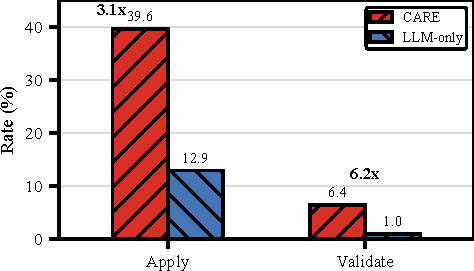
\includegraphics[width=\columnwidth]{img/care_eval_yield.pdf}
  \caption{Patch apply and validation pass rates for \SysName{} and LLM-only on
  487 critical findings. Both systems use the same LLM-call budget.}
  \label{fig:eval-yield}
\end{figure}

The validation gap is larger. \SysName{} obtains 31 fully validated patches,
whereas LLM-only obtains 5. This is a 6.2$\times$ improvement in validation pass
rate. The main reason is not simply that \SysName{} asks the model for a better
diff. The system constrains generation with resource and behavior-preservation
invariants, converts JSON edit plans into diffs when possible, repairs common
path mistakes, and rejects candidates that do not preserve resource lifecycle
facts. These implementation choices turn the LLM into a patch proposal engine
whose outputs are filtered by concrete project behavior and security checks.

The gain remains visible after conditioning on patches that apply. Among
applicable patches, \SysName{} validates 31 of 193 candidates, while LLM-only
validates 5 of 63. Thus, \SysName{} improves both stages of the pipeline: it
helps the model produce patches that can be materialized in the target tree, and
it gives the model enough safety context to produce a larger number of patches
that survive validation. In absolute terms, \SysName{} produces 26 more
validated patches than LLM-only with the same number of LLM calls.

The absolute pass rate should be interpreted as a fail-closed yield rather than
as an attempt to accept every plausible edit. Critical resource-lifecycle
findings often involve ownership and cleanup conditions that are difficult to
establish locally. \SysName{} therefore rejects any candidate that cannot pass
the complete validator. Under this conservative acceptance policy, the system
still produces substantially more validated patches than direct LLM-only
patching.

\subsection{Validator Ablation}
\label{sec:evaluation-ablation}

Table~\ref{tab:eval-ablation} shows why the full validator is necessary. With
the full \SysName{} validator, 31 patches pass. If the resource checker is
removed, 189 patches would pass, adding 158 extra accepted patches. The
LLM-assisted review classifies 121 of these extra accepts as false accepts,
yielding a 76.58\% false-accept rate among the extra accepted patches. Removing
all three lightweight regression checkers has a similar effect: the pass count
rises to 193, but 125 extra patches are judged false accepts.

\begin{table}[t]
  \centering
  \caption{Validator ablation for \SysName{} on critical findings.}
  \label{tab:eval-ablation}
  \footnotesize
  \begin{tabular}{@{}lrrr@{}}
    \toprule
    \textbf{Variant} & \textbf{Passed} & \textbf{Extra} & \textbf{False} \\
    \midrule
    Full validator & 31 & 0 & 0 \\
    No resource checker & 189 & 158 & 121 \\
    No semantic checker & 31 & 0 & 0 \\
    No security checker & 32 & 1 & 1 \\
    No resource/semantic/security & 193 & 162 & 125 \\
    \bottomrule
  \end{tabular}
\end{table}

Figure~\ref{fig:eval-ablation} shows the same ablation visually. The taller bars
in the ablated configurations are not improvements: the red portions are
review-identified false accepts that the full validator prevents.

\begin{figure}[t]
  \centering
  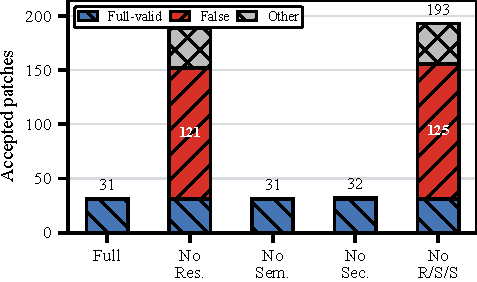
\includegraphics[width=\columnwidth]{img/care_eval_ablation.pdf}
  \caption{Validator ablation for \SysName{}. Removing resource and security
  gates increases the number of accepted patches mainly by admitting false
  accepts.}
  \label{fig:eval-ablation}
\end{figure}

This result supports the central design claim of \SysName{}: build and test
success alone are not enough for security-aware refactoring. In this workload,
the resource checker carries most of the safety burden because the queue
contains critical resource-imbalance findings. A patch can compile, apply
cleanly, and leave function signatures unchanged while still failing to repair a
double free, adding a cleanup operation on the wrong path, or leaving an early
return that bypasses cleanup. The semantic checker does not change this
particular critical-resource queue, but it remains part of the full validator
because other refactoring categories, such as duplicate-check removal and
cleanup consolidation, can alter return forms or externally visible calls.

The ablation also quantifies the validator's precision role. Without resource
checking, the apparent pass rate rises from 6.37\% to 38.81\%, but most of this
increase is unsafe. In other words, the additional accepted patches are not
latent successes; they are candidates that the full system correctly prevents
from reaching the user as selected refactorings. This is the main empirical
evidence that \SysName{} should be evaluated by validated output rather than by
LLM generation alone.

A representative safety case illustrates the point. In one FLAC candidate, the
LLM added a null assignment after a free. The patch applied and passed the
non-resource stages, but the resource checker still reported an unresolved
double-free pattern. Without the resource checker, such a patch would look
acceptable to a syntax- and build-oriented pipeline. With the full validator, it
is rejected and the failure is converted into repair feedback.

\subsection{Patch Quality and Safety Evidence}
\label{sec:evaluation-review}

We review accepted patches using a second-pass LLM-assisted review protocol.
For accepted patches, the review classifies a patch as
\emph{correct}, \emph{likely correct}, \emph{incorrect}, or \emph{uncertain}.
We separately use the same review workflow to inspect validator-rejected
candidates during ablations, which helps distinguish true missed opportunities
from unsafe false accepts.

\begin{table}[t]
  \centering
  \caption{LLM-assisted review of validator-accepted patches.}
  \label{tab:eval-review}
  \footnotesize
  \begin{tabular}{@{}lrrrr@{}}
    \toprule
    \textbf{System} & \textbf{Reviewed} & \textbf{Correct} & \textbf{Likely} & \textbf{Bad} \\
    \midrule
    \SysName{} & 31 & 7 & 24 & 0 \\
    LLM-only & 5 & 2 & 3 & 0 \\
    \bottomrule
  \end{tabular}
\end{table}

All validator-accepted patches were classified as correct or likely correct by
the reviewer. For \SysName{}, 7 of 31 accepted patches were classified as
strictly correct and the remaining 24 as likely correct. For LLM-only, 2 of 5
were classified as correct and 3 as likely correct. This result should be read
as supporting evidence for the validator rather than a replacement for human
review: the reviewer provides consistent triage, but the validator provides the
hard acceptance criterion.

The accepted-patch review is important because the validator is intentionally
strict. A patch can be syntactically small and plausible but still fail if it
does not repair the reported lifecycle issue or if it weakens a security check.
The zero-invalid result among accepted patches suggests that the validation
pipeline is a useful final filter: it sacrifices speculative acceptance in
exchange for a cleaner selected-patch set.

The positive cases are small and security-relevant. In one cJSON finding,
\SysName{} added a missing \texttt{cJSON\_Delete(object4)} call in a test utility
cleanup path. The patch applied, compiled, passed the resource checker, passed
semantic and security regression checks, and was classified as likely correct by
the review. The LLM-only patch for the same finding did not pass validation.
This case captures the intended workflow: detector evidence identifies a
resource-lifecycle problem, the LLM proposes a minimal edit, and the validator
accepts it only after the resource and regression checks agree.

A second safety-oriented case shows the benefit of validation even when a patch
looks reasonable. A generated edit that merely nulls a pointer after a free can
make local code appear tidier without actually removing a double-release path.
\SysName{} rejects such candidates because the resource checker compares the
post-patch lifecycle facts rather than the surface form of the edit. Together,
the accepted-patch review and validator ablation show that the system is useful
not only for producing patches, but also for preventing unsafe patches from
being reported as successes.

\subsection{Scalability and Cost}
\label{sec:evaluation-scalability}

Table~\ref{tab:eval-cost} summarizes the scalability results. The dry scan over
OSS50 required no LLM calls and took 8,359.842 aggregate seconds, with a median
of 29.776 seconds per project and a p95 of 1,360.238 seconds. The critical
\SysName{} patch/validation run made 487 LLM calls, one per opportunity, with a
mean candidate runtime of 94.3 seconds and a median of 30.283 seconds. The
LLM-only run used the same number of LLM calls and had a similar per-candidate
runtime, but produced far fewer validated patches.

\begin{table}[t]
  \centering
  \caption{Cost and scalability summary.}
  \label{tab:eval-cost}
  \scriptsize
  \begin{tabular}{@{}p{0.38\columnwidth}rrr@{}}
    \toprule
    \textbf{Phase} & \textbf{Items} & \textbf{LLM} & \textbf{Med. s} \\
    \midrule
    OSS50 dry scan & 50 & 0 & 29.776 \\
    \SysName{} critical val. & 487 & 487 & 30.283 \\
    LLM-only critical val. & 487 & 487 & 34.197 \\
    Patch review & 974 & 115 & -- \\
    Detector review & 100 & 10 & -- \\
    \bottomrule
  \end{tabular}
\end{table}

These results show that \SysName{} separates cheap discovery from expensive
patch validation. The detector scan can run over tens of thousands of files
without invoking an LLM. LLM calls are reserved for selected high-priority
findings, and the validation scripts are resumable so long-running runs can be
restarted without losing completed work. For parallel execution, the
project-sharded runner prevents two processes from mutating the same project,
while the dynamic runner drains remaining work items in isolated per-worker
copies. The runtime is therefore dominated by LLM latency, patch application,
and project-specific build/test cost rather than by the Python orchestration
itself.

The cost profile is favorable for practical use. A user can run the dry scan
over an entire project collection without spending LLM budget, inspect or rank
the resulting opportunities, and then spend real LLM calls only on the subset
that matters for a study or maintenance task. In the completed critical queue,
\SysName{} and LLM-only spend the same 487 LLM calls, but \SysName{} returns
more applicable patches and more validated patches. This means the additional
analysis and validation machinery improves the value obtained per LLM call.

Overall, the evaluation supports three claims. First, adding program context and
structured safety contracts substantially improves patch applicability and
validated-patch yield over direct LLM-only patching. Second, resource-aware
validation is essential: without it, many unsafe patches would be accepted.
Third, the prototype is already scalable enough to scan large C/C++ project
sets and to run real LLM validation on prioritized queues. The main takeaway is
that \SysName{} changes the role of the LLM from an untrusted editor into a
proposal component embedded inside a security-aware validation loop.
